%!TEX program = xelatex
\documentclass[12pt,a4paper]{article}

\usepackage{polyglossia}

\setdefaultlanguage[variant=mono]{greek}
\setotherlanguage{english}
\setmainfont{GFS Elpis}
\newfontfamily{\greekfont}{GFS Elpis}
\newfontfamily{\latinfont}{GFS Elpis}
\newfontfamily{\greekfonttt}{Cascadia Code}


\usepackage{listings}
\usepackage{float}
\usepackage{graphicx}
\usepackage{amsmath}
\usepackage{amsfonts}
\usepackage{amssymb}
\usepackage{hyperref}


\author{Γραμμένος Θεόδωρος} 
\title{Σήματα-Συστήματα\\Προγραμματιστικό Θέμα}
\date{Α.Ε.Μ.: 3294}
\begin{document}
    \maketitle
    \section{Τεχνικές Πληροφορίες}
    Η εργασία υλοποιήθηκε στη γλώσσα C++ με το build system CMake.
    Ο κώδικας χωρίζεται σε 2 κομμάτια:
    \begin{itemize}
        \item Ο κώδικας που υλοποιεί τα ζητούμενα της άσκησης βρίσκεται στους φακέλους src και include
        \item Οι βοηθητικές συναρτήσεις υλοποιούνται στη βιβλιοθήκη που βρίσκεται στον υποφάκελο Helper
    \end{itemize}
    Για την ανάγνωση και την εγγραφή των αρχείων wav χρησιμοποιείται η βιβλιοθήκη libsndfile
    (\url{https://github.com/libsndfile/libsndfile}). Επιπλέον, στην εργασία περιλαμβάνεται η βιβλιοθήκη 
    GoogleTest προκειμένου να ελεγχθεί η σωστή λειτουργία των συναρτήσεων.

    \section{Helper}
    \subsection{UI.h/UI.cpp}
    Στα αρχεία αυτά ορίζονται μέθοδοι που έχουν σχέση με την επικοινωνία με τον χρήστη.
    \begin{itemize}
        \item Η συνάρτηση getIntLargerThan ζητάει από το χρήστη μία τιμή μεγαλύτερη από αυτή που δίνεται ως παράμετρος.
        \item Η συνάρτηση formatVector δέχεται ως είσοδο ένα vector και επιστρέφει την αναπαράστασή του ως string.
    \end{itemize}
    \subsection{Utils.h}
    Στο αρχείο περιλαμβάνονται βοηθητικές συναρτήσεις
    \begin{itemize}
        \item Η συνάρτηση createRandomVector δημιουργεί ένα vector τυχαίων αριθμών του τύπου και του μεγέθους που δίνεται.
        \item Η συνάρτηση normalize δέχεται ως είσοδο ένα vector και κανονικοποιεί τα στοιχεία του στο [-1,1].
    \end{itemize}

    \subsection{Κύριο πρόγραμμα}
    \subsubsection{myConvolve.h}
    Στο αρχείο αυτό υλοποιούνται οι συναρτήσεις που έχουν σχέση με τη συνέλιξη. \par
    Δημιουργήθηκαν δύο υλοποιήσεις της συνέλιξης: στη συνάρτηση singleConvolve υλοποιείται ο αλγόριθμος σύμφωνα με τον ορισμό 
    της συνέλιξης σε ένα thread. Λόγω της αργής ταχύτητας της συγκεκριμένης υλοποίησης δημιουργήθηκε η συνάρτηση myConvolve η 
    οποία εκτελεί τη συνέλιξη παράλληλα σε διαφορετικά threads. Αυτό το επιτυγχάνει χρησιμοποιώντας τη συνάρτηση convolveAtRange 
    η οποία δέχεται δύο vectors, τα σήματα στα οποία γίνεται η συνέλιξη, και δύο αριθμούς start και end και υπολογίζει τα αποτελέσματα 
    της συνέλιξης για τα $n$ στο διάστημα $[start,end]$. \par
    Για να ελεγχθεί ότι η συνάρτηση myConvolve δουλεύει σωστά δημιουργήθηκαν κάποια unit tests τα οποία βρίσκονται στο αρχείο test/Convolution.cpp.
    Για τα tests δημιουργήθηκαν κάποια τυχαία σήματα και υπολογίστηκε η συνέλιξή τους μέσω MATLAB. Στα tests ελέγχεται ότι η συνάρτηση 
    myConvolve δουλεύει ανεξάρτητα από το σχετικό μέγεθος των σημάτων που δίνονται ως είσοδος και επιστρέφει το σωστό αποτέλεσμα.
    \subsubsection{ex2.cpp}
    Στο αρχείο αυτό υλοποιούνται οι συναρτήσεις που έχουν σχέση με τη 2η άσκηση. \par
    Για το πρώτο ερώτημα, δημιουργήθηκε η επιπλέον συνάρτηση convertToMono η οποία δέχεται τα δεδομένα ενός πολυκαναλικού WAV σήματος και 
    διατηρεί μόνο το πρώτο κανάλι. Αυτό έγινε γιατί το αρχείο pink\_noise.wav έχει δύο κανάλια ενώ το sample\_audio.wav μόνο ένα. Το ζητούμενο του 
    πρώτου ερωτήματος υλοποιείται στη συνάρτηση question1.\par
    Για το δεύτερο ερώτημα δημιουργήθηκε η συνάρτηση createWhiteNoiseSignal η οποία παράγει ένα σήμα λευκού θορύβου παίρνοντας τυχαίους 
    αριθμούς που ακολουθούν κανονική κατανομή. Το ζητούμενο του 2ου ερωτήματος υλοποιείται στη συνάρτηση question2.
    \subsection{Παράδειγμα}
    Τρέχουμε τη συνάρτηση question1 και δίνουμε ως input 11.
    \begin{figure}[H]
        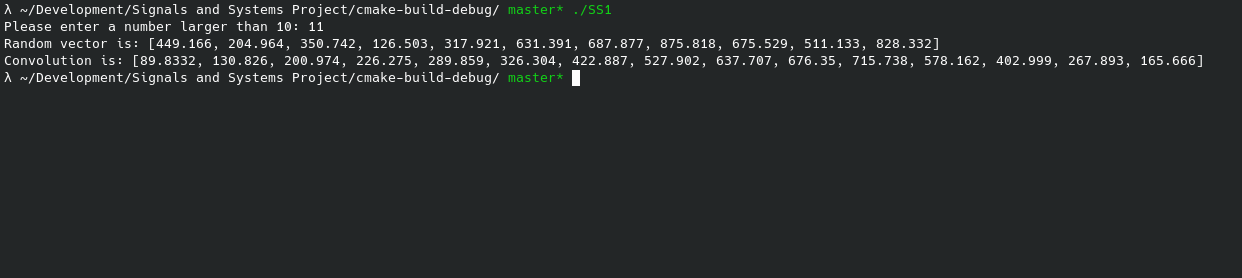
\includegraphics[width=\linewidth]{res1.png}
        \caption{Αποτέλεσμα της εκτέλεσης του προγράμματος}
    \end{figure}
    Το πρόγραμμα δείχνει το τυχαίο σήμα που δημιουργήθηκε καθώς και το αποτέλεσμα της συνέλιξης με το σήμα της εκφώνησης.
    Εκτελώντας τη συνέλιξη με τα ίδια σήματα στο MATLAB μπορούμε να δούμε ότι το αποτέλεσμα είναι σωστό. Μόνο μερικά δεκαδικά ψηφία 
    διαφέρουν λόγω της στρογγυλοποίησης.
    \begin{figure}[H]
        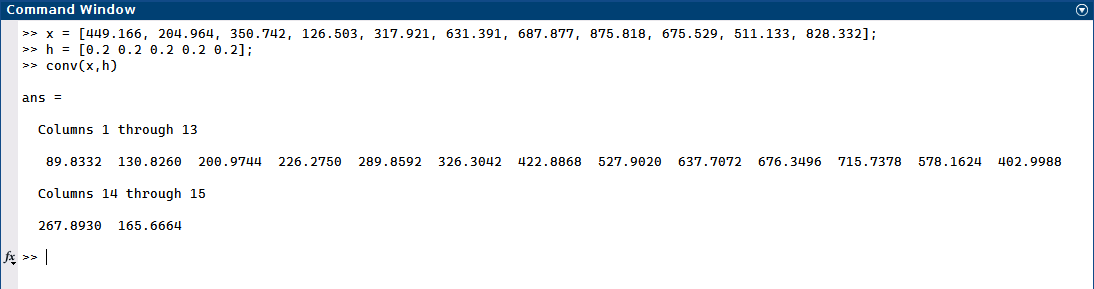
\includegraphics[width=\linewidth]{res2.png}
        \caption{Αποτέλεσμα εκτέλεσης της συνέλιξης στο MATLAB}
    \end{figure}
\end{document}